% Provenance (never printed): cycle 2 "Questionner le monde de la matiere"
% (solid materials, observing and sorting) and cycle 3 theme 4 (local geology,
% rocks for building); see sources/book1/PROVENANCE.md. Book 1, grade 3, ch. 1.
\chapter{Stenen, kiezels en zand}\label{ch:g3:stones-pebbles-sand}

Tom is op vakantie bij een \omterm{def:g1:landscapes-around-us:water}{rivier}. Op de grindbank, waar het water ondiep
is, raapt hij een kiezelsteen op. Die is glad en rond, bijna als een ei, en
past precies in zijn hand. Vorige week, toen hij met zijn ouders over een
bergpad hoog in hetzelfde \omterm{def:g1:landscapes-around-us:landform}{dal} liep, zag hij stenen met dezelfde kleur onder
een rotsachtige helling liggen --- maar die stenen waren scherp, met randen
en hoeken.

Hoe is een scherpe steen van de \omterm{def:g1:landscapes-around-us:landform}{berg} beneden in het \omterm{def:g1:landscapes-around-us:landform}{dal} een gladde, ronde
\omterm{def:g3:stones-pebbles-sand:pebble}{kiezel} geworden? Om dat uit te zoeken, beginnen we bij het \omterm{def:g3:stones-pebbles-sand:rock}{gesteente} zelf.

\begin{omfigure}
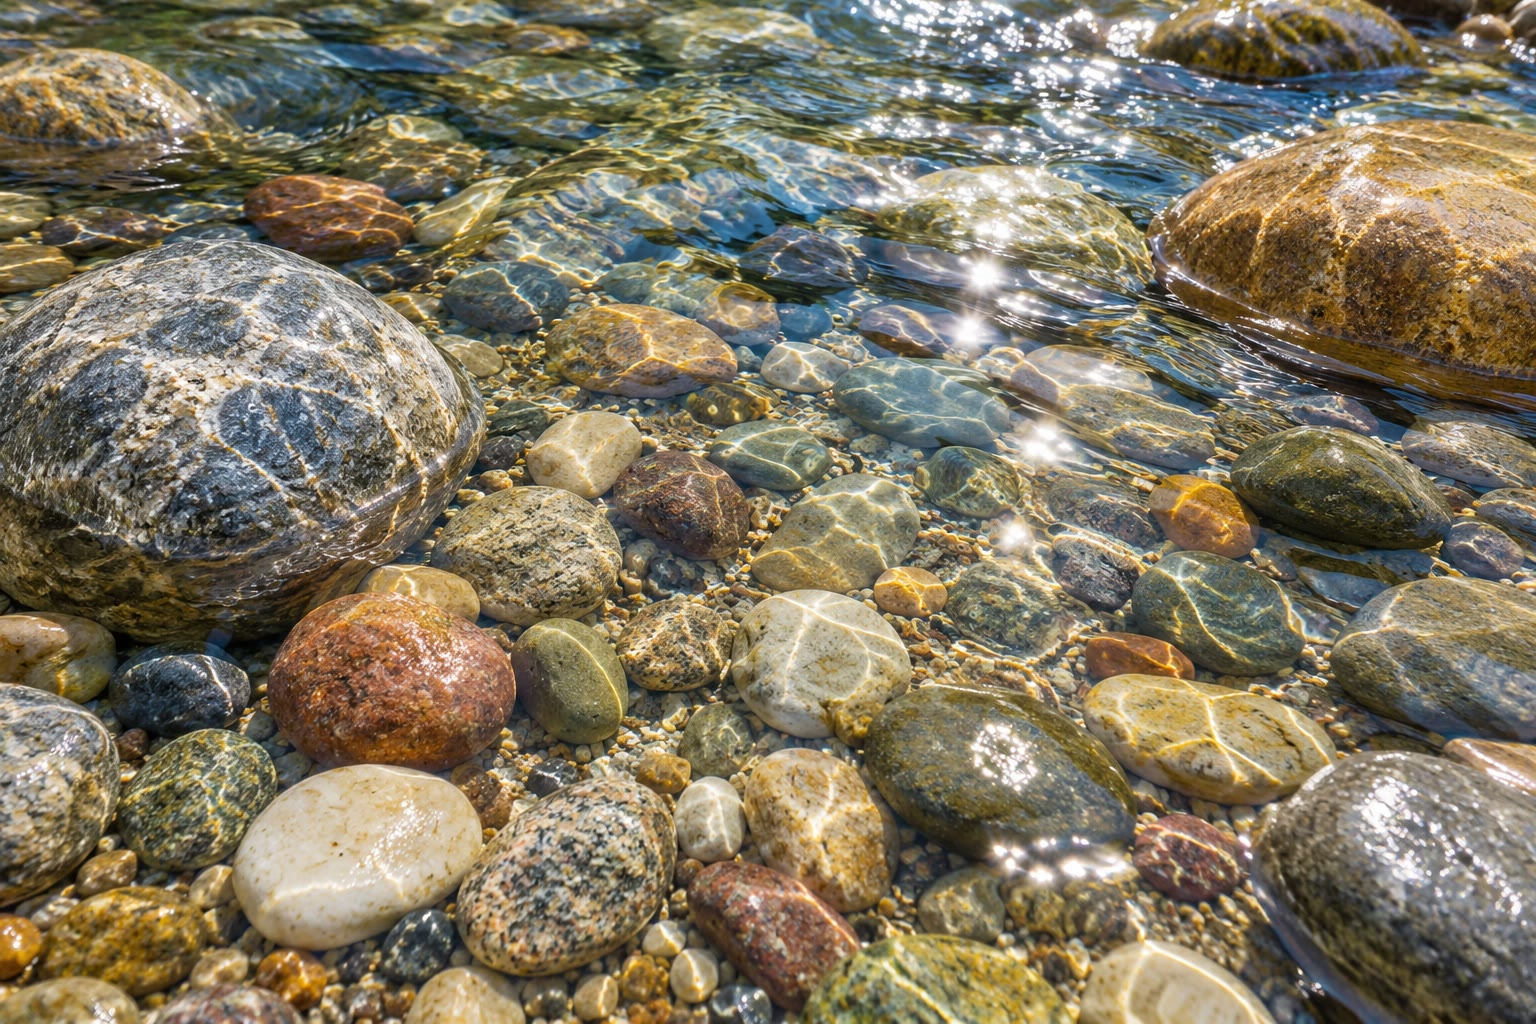
\includegraphics[width=0.62\linewidth]{images/book1/ai/g3-stream-pebbles.jpg}

{\small Ronde \omterm{def:g3:stones-pebbles-sand:pebble}{kiezels} onder het heldere water van een beek.}
\end{omfigure}

\begin{recall}
In een \omterm{def:g1:landscapes-around-us:landscape}{landschap} zijn er \omterm{def:g1:landscapes-around-us:landform}{bergen}, \omterm{def:g1:landscapes-around-us:landform}{heuvels}, \omterm{def:g1:landscapes-around-us:landform}{dalen} en \omterm{def:g1:landscapes-around-us:landform}{vlakten}, en \omterm{def:g1:landscapes-around-us:water}{rivieren} die
van het hoge land naar beneden stromen, naar de \omterm{def:g2:water-on-earth:ocean}{zee}
(\cref{ch:g1:landscapes-around-us}). De bovenste laag van de grond, waarin
planten groeien, is de bodem: de biologieboeken vertellen hoe levende wezens
die maken.
\end{recall}

\section{Gesteente: de harde grond onder onze voeten}

Graaf een diep gat in een tuin. Eerst vind je donkere, zachte aarde met
wortels erin. Daaronder wordt de grond lichter en steniger. En als je diep
genoeg kon graven, zou je altijd bij iets hards komen dat een schep niet
kan doorsteken: \omterm{def:g3:stones-pebbles-sand:rock}{gesteente}.

\begin{definition}[Gesteente en vast gesteente]\label{def:g3:stones-pebbles-sand:rock}
Een \emph{gesteente}\index{gesteente} is een hard, natuurlijk materiaal
waaruit de vaste Aarde bestaat. Het \emph{vaste
gesteente}\index{vast gesteente} is het harde gesteente dat overal op het
land onder de bodem ligt, en onder het \omterm{def:g3:stones-pebbles-sand:sand}{zand} en het \omterm{def:g3:stones-pebbles-sand:sand}{slib} van de zeebodem.
\end{definition}

Op de meeste plaatsen is het \omterm{def:g3:stones-pebbles-sand:rock}{vaste gesteente} verborgen onder de bodem, het
gras en de bomen. We zien het waar geen bodem is om het te bedekken: op de
steile flanken van \omterm{def:g1:landscapes-around-us:landform}{bergen}, in kliffen aan \omterm{def:g2:water-on-earth:ocean}{zee} en langs wegen die door een
\omterm{def:g1:landscapes-around-us:landform}{heuvel} zijn uitgegraven.

\begin{omfigure}
\begin{tikzpicture}[x=1cm, y=1cm, font=\small]
  % bedrock
  \fill[omLithGranite!60] (0,0) rectangle (11,2.2);
  \foreach \x/\y in {0.6/0.5, 1.8/1.4, 3.1/0.7, 4.4/1.6, 5.6/0.4, 6.9/1.2, 8.3/0.6, 9.6/1.5, 10.3/0.4}
    \draw[black!40, line width=0.4pt] (\x,\y) -- ++(0.5,0.25);
  % soil (thick on the left, missing on the steep right)
  \fill[brown!55] (0,2.2) -- (0,3.4) .. controls (2,3.5) and (4,3.4) .. (5.6,3.2) -- (6.4,2.9) -- (6.4,2.2) -- cycle;
  \fill[brown!30] (0,2.2) rectangle (6.4,2.65);
  % rock showing on the right: a hill side with no soil
  \fill[omLithGranite!60] (6.4,2.2) -- (6.4,2.9) -- (7.6,3.9) -- (8.8,4.3) -- (11,4.3) -- (11,2.2) -- cycle;
  \draw[black!60] (0,3.4) .. controls (2,3.5) and (4,3.4) .. (5.6,3.2) -- (6.4,2.9) -- (7.6,3.9) -- (8.8,4.3) -- (11,4.3);
  % grass and roots
  \foreach \x in {0.3,0.8,...,5.3}
    \draw[green!50!black, line width=0.6pt] (\x,{3.4-0.04*\x}) -- ++(0.05,0.18);
  \foreach \x in {1.2,3.4,4.9}
    \draw[brown!80!black, line width=0.5pt] (\x,3.3) -- ++(-0.1,-0.5) -- ++(0.15,-0.3);
  % labels
  \node[anchor=west] at (11.2,3.6) {gesteente aan};
  \node[anchor=west] at (11.2,3.2) {het oppervlak};
  \draw[black!60] (11.15,3.4) -- (9.6,4.15);
  \node[anchor=east] at (-0.2,2.9) {bodem};
  \draw[black!60] (-0.15,2.9) -- (0.6,2.9);
  \node[anchor=west] at (11.2,1.1) {vast gesteente};
  \draw[black!60] (11.15,1.1) -- (10.6,1.1);
\end{tikzpicture}

{\small Een doorsnede van de grond. Onder de bodem zit altijd het \omterm{def:g3:stones-pebbles-sand:rock}{vaste
gesteente}. Op de steile heuvelflank, rechts, ontbreekt de bodem en komt het
\omterm{def:g3:stones-pebbles-sand:rock}{gesteente} aan het oppervlak.}
\label{fig:g3:stones-pebbles-sand:ground}
\end{omfigure}

\section{Van gesteente tot kiezels}

\omterm{def:g3:stones-pebbles-sand:rock}{Gesteente} is hard, maar het blijft niet eeuwig bestaan. In de winter dringt
water in de spleten van een rots; het bevriest, zet uit en duwt de spleten
wijder open. Ook wortels groeien in spleten. Beetje bij beetje breken er
stukken af die naar beneden vallen: daar komen de scherpe stenen onder de
berghellingen vandaan.

Als een scherpe steen in een bergbeek valt, rolt het water hem over de
bodem, stoot hem tegen andere stenen en sleept hem over \omterm{def:g3:stones-pebbles-sand:sand}{zand}. Zijn hoeken
slijten het eerst af. Hoe verder hij reist, hoe ronder en gladder hij
wordt. Tegen de tijd dat hij beneden in het \omterm{def:g1:landscapes-around-us:landform}{dal} aankomt, is hij een \omterm{def:g3:stones-pebbles-sand:pebble}{kiezel}
geworden.

\begin{definition}[Kiezel en grind]\label{def:g3:stones-pebbles-sand:pebble}
Een \emph{kiezel}\index{kiezel} is een klein stuk \omterm{def:g3:stones-pebbles-sand:rock}{gesteente} dat rond en
glad is geworden doordat water het voortrolde, in een \omterm{def:g1:landscapes-around-us:water}{rivier} of op een
strand. \emph{Grind}\index{grind} is een hoop kleine stenen en kiezels bij
elkaar, met korrels die groter zijn dan zandkorrels.
\end{definition}

\begin{omfigure}
\begin{tikzpicture}[x=1cm, y=1cm, font=\small]
  \draw[ocBlue!70!black, line width=1.2pt, -{Stealth[length=3mm]}] (0,0) -- (12.2,0);
  \node[below, font=\scriptsize] at (6.1,-0.15) {de beek voert de steen naar beneden, bij elk hoog water een stukje verder};
  \foreach \x/\shape/\t in {
     0.8/{(-0.55,-0.1) -- (-0.2,0.5) -- (0.35,0.55) -- (0.6,0.05) -- (0.3,-0.45) -- (-0.35,-0.5) -- cycle}/van de rots gevallen,
     4.0/{(-0.5,-0.1) [rounded corners=4pt] -- (-0.2,0.45) -- (0.3,0.5) -- (0.55,0.05) -- (0.3,-0.4) -- (-0.35,-0.45) -- cycle}/hoeken afgesleten,
     7.2/{(-0.45,-0.05) [rounded corners=8pt] -- (-0.15,0.42) -- (0.3,0.45) -- (0.5,0.05) -- (0.3,-0.35) -- (-0.3,-0.4) -- cycle}/ronder en kleiner,
     10.4/{(0,0) ellipse (0.45 and 0.3)}/een gladde kiezel} {
    \begin{scope}[shift={(\x,1.1)}]
      \fill[omLithGranite!80, draw=black!70] \shape;
    \end{scope}
    \node[font=\scriptsize] at (\x,0.35) {\t};
  }
\end{tikzpicture}

{\small De reis van een steen in een \omterm{def:g1:landscapes-around-us:water}{rivier}: scherp als hij van de rots
valt, rond en glad na een lange tocht stroomafwaarts.}
\label{fig:g3:stones-pebbles-sand:journey}
\end{omfigure}

\begin{remark}[De vorm van een steen lezen]\label{rem:g3:stones-pebbles-sand:shape}
De vorm van een steen vertelt zijn verhaal. Een scherpe steen heeft nog
niet ver gereisd van de rots waar hij van afbrak. Een ronde, gladde \omterm{def:g3:stones-pebbles-sand:pebble}{kiezel}
is lang door water voortgerold, in een \omterm{def:g1:landscapes-around-us:water}{rivier} of door de golven van de \omterm{def:g2:water-on-earth:ocean}{zee}.
\end{remark}

\section{Zand en slib}

De stenen en \omterm{def:g3:stones-pebbles-sand:pebble}{kiezels} die tegen elkaar botsen, slaan ook piepkleine
stukjes van elkaar af. Na heel lange tijd worden die stukjes \omterm{def:g3:stones-pebbles-sand:sand}{zand}. Bekijk
\omterm{def:g3:stones-pebbles-sand:sand}{zand} eens door een vergrootglas: elke korrel is een stukje \omterm{def:g3:stones-pebbles-sand:rock}{gesteente}, of
een stukje schelp, en vaak ook afgerond.

\begin{definition}[Zand en slib]\label{def:g3:stones-pebbles-sand:sand}
% ledger: usgs:wentworth
\emph{Zand}\index{zand} bestaat uit losse korrels gebroken \omterm{def:g3:stones-pebbles-sand:rock}{gesteente} die
kleiner zijn dan 2 millimeter: we kunnen elke korrel nog zien.
\emph{Slib}\index{slib} bestaat uit korrels die zo klein zijn dat we ze
niet een voor een kunnen zien; nat is het zacht en plakkerig, zoals modder.
\end{definition}

Geologen sorteren stukken gebroken \omterm{def:g3:stones-pebbles-sand:rock}{gesteente} op grootte, van groot naar
klein: rotsblokken, \omterm{def:g3:stones-pebbles-sand:pebble}{kiezels} en \omterm{def:g3:stones-pebbles-sand:pebble}{grind}, \omterm{def:g3:stones-pebbles-sand:sand}{zand}, en \omterm{def:g3:stones-pebbles-sand:sand}{slib}.

\begin{omfigure}
\begin{tikzpicture}[x=1mm, y=1mm, font=\small]
  % true size: 1 unit = 1 mm
  \draw[black!40] (0,-14) -- (150,-14);
  \foreach \x in {0,10,...,150} \draw[black!40] (\x,-14) -- (\x,-12.5);
  \foreach \x in {0,50,100,150} \node[font=\scriptsize, below] at (\x,-14.5) {\pgfmathparse{int(\x/10)}\pgfmathresult\,cm};
  % mud: too small
  \node[font=\scriptsize, align=center] at (6,14) {slib};
  \fill[brown!60] (6,0) circle (0.05);
  \node[font=\scriptsize, align=center] at (6,4.5) {korrels te\\klein om te zien};
  % sand grains: up to 2 mm
  \node[font=\scriptsize] at (28,14) {zand};
  \foreach \x/\r in {22/0.3, 25/0.5, 28/0.75, 32/1.0}
    \fill[yellow!60!brown, draw=black!50, line width=0.2pt] (\x,0) circle (\r);
  \node[font=\scriptsize, align=center] at (28,5) {kleiner dan\\2 millimeter};
  % gravel and pebbles
  \node[font=\scriptsize] at (78,22) {grind en kiezels};
  \fill[omLithGranite!80, draw=black!60] (52,0) ellipse (2 and 1.5);
  \fill[black!25, draw=black!60] (62,0) ellipse (4 and 3);
  \fill[omLithGranite!80, draw=black!60] (78,0) ellipse (8 and 6);
  \fill[black!30, draw=black!60] (104,0) ellipse (15 and 10);
  % boulder: off scale
  \node[font=\scriptsize] at (138,22) {rotsblok};
  \fill[black!20, draw=black!60] (128,-10) .. controls (127,8) and (135,16) .. (142,15) .. controls (150,14) and (152,4) .. (149,-10) -- cycle;
  \node[font=\scriptsize, align=center, fill=white, fill opacity=0.7, text opacity=1, inner sep=1pt] at (139,4) {veel te klein\\getekend};
\end{tikzpicture}

{\small Korrels gebroken \omterm{def:g3:stones-pebbles-sand:rock}{gesteente}, van de kleinste tot de grootste. \omterm{def:g3:stones-pebbles-sand:sand}{Slib},
\omterm{def:g3:stones-pebbles-sand:sand}{zand}, \omterm{def:g3:stones-pebbles-sand:pebble}{grind} en \omterm{def:g3:stones-pebbles-sand:pebble}{kiezels} zijn op ware grootte getekend: vergelijk ze met een
liniaal. Een rotsblok kan zo groot zijn als een stoel, of als een huis.}
\label{fig:g3:stones-pebbles-sand:sizes}
\end{omfigure}

\begin{omfigure}
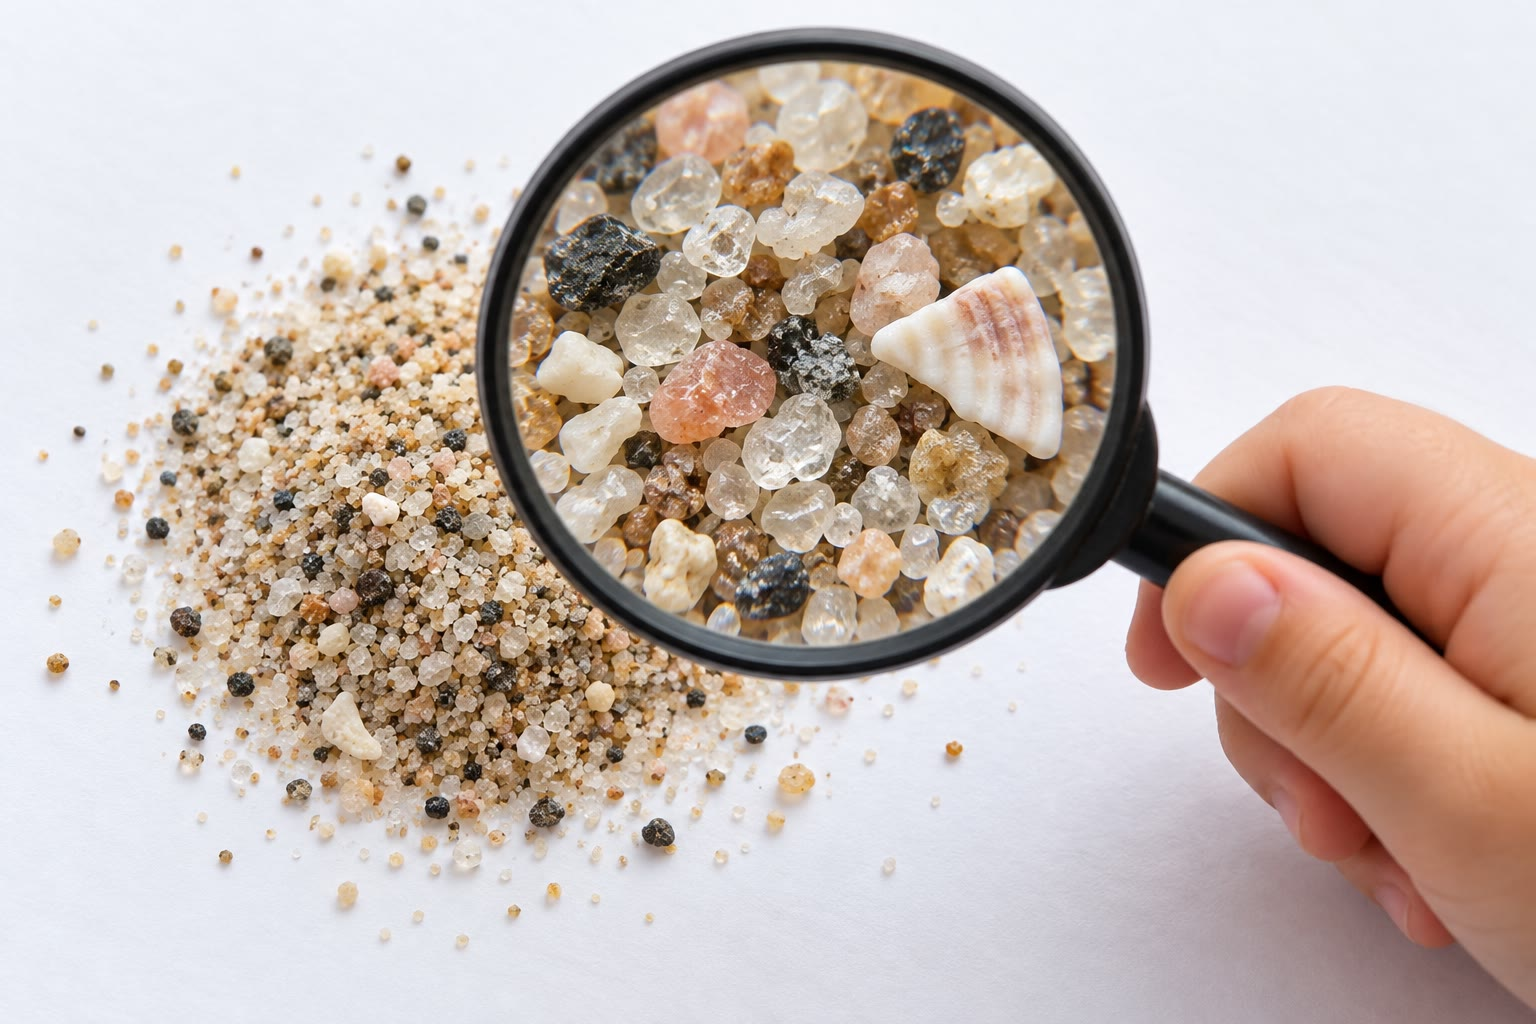
\includegraphics[width=0.55\linewidth]{images/book1/ai/g3-sand-magnifier.jpg}

{\small Strandzand door een vergrootglas: piepkleine korrels \omterm{def:g3:stones-pebbles-sand:rock}{gesteente} en
stukjes schelp.}
\end{omfigure}

\begin{method}[Gebroken gesteente op grootte sorteren]\label{met:g3:stones-pebbles-sand:sort}
Om een stuk gebroken \omterm{def:g3:stones-pebbles-sand:rock}{gesteente} een naam te geven, kijk je naar zijn grootte:
\begin{enumerate}
  \item kun je de korrels niet zien, zelfs niet van dichtbij, dan is het
        \omterm{def:g3:stones-pebbles-sand:sand}{slib};
  \item kun je elke korrel zien, maar is elke korrel kleiner dan
        2 millimeter (de dikte van een munt), dan is het \omterm{def:g3:stones-pebbles-sand:sand}{zand};
  \item zijn de stukken groter, maar kun je er één in je hand houden, dan
        zijn het \omterm{def:g3:stones-pebbles-sand:pebble}{grind} en \omterm{def:g3:stones-pebbles-sand:pebble}{kiezels};
  \item is een stuk te zwaar om op te tillen, dan is het een rotsblok.
\end{enumerate}
\end{method}

\begin{example}[Waar vinden we elke grootte?]\label{ex:g3:stones-pebbles-sand:where}
Snel water kan grote stenen meevoeren; langzaam water laat ze vallen en
neemt alleen kleine korrels mee. Daarom liggen rotsblokken en scherpe
stenen in de steile bergbeken, \omterm{def:g3:stones-pebbles-sand:pebble}{kiezels} en \omterm{def:g3:stones-pebbles-sand:pebble}{grind} op de oevers van de \omterm{def:g1:landscapes-around-us:water}{rivier}
in het \omterm{def:g1:landscapes-around-us:landform}{dal}; \omterm{def:g3:stones-pebbles-sand:sand}{zand} verzamelt zich op stranden en in rustige bochten van de
\omterm{def:g1:landscapes-around-us:water}{rivier}, en \omterm{def:g3:stones-pebbles-sand:sand}{slib} zakt neer waar het water bijna stilstaat, in vijvers, \omterm{def:g1:landscapes-around-us:water}{meren}
en riviermondingen.
\end{example}

\section{Harde en zachte gesteenten}

Niet alle \omterm{def:g3:stones-pebbles-sand:rock}{gesteenten} zijn even hard. Sommige, zoals graniet, zijn zo hard
dat ze glas krassen en duizenden jaren meegaan in een muur. Andere
brokkelen af in je hand, zoals krijt, dat een witte streep op een bord
achterlaat. Sommige \omterm{def:g3:stones-pebbles-sand:rock}{gesteenten} bestaan uit korrels die we kunnen zien;
andere zijn glad en zien er van de ene kant tot de andere hetzelfde uit.

\begin{example}[Drie gesteenten vergeleken]\label{ex:g3:stones-pebbles-sand:three}
\emph{Graniet} is gespikkeld met roze, witte en zwarte korrels en is heel
hard. \emph{Zandsteen} bestaat uit zandkorrels die aan elkaar vastzitten;
als je erover wrijft, laat hij soms een paar korrels los. \emph{Krijt} is
wit, zacht en poederig. In een later jaar leer je hoe elk van deze
\omterm{def:g3:stones-pebbles-sand:rock}{gesteenten} is ontstaan.
\end{example}

\begin{omfigure}
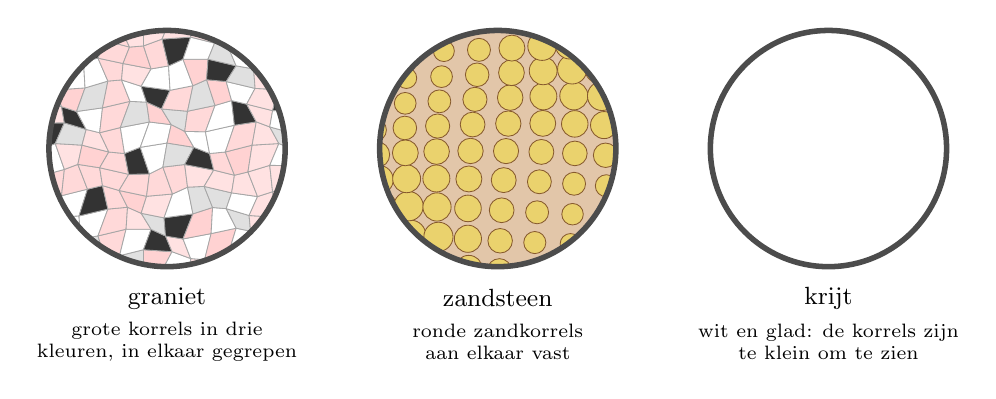
\begin{tikzpicture}[font=\small]
  % three stones seen through a magnifying glass (drawn, not to scale)
  % granite: interlocking grains of three colours
  \begin{scope}
    \clip (0,0) circle (1.5);
    % a jittered lattice: the cells tile the disk with no gap, like the
    % interlocking crystals of granite
    \foreach \i in {-6,...,5} \foreach \j in {-6,...,5} {
      \pgfmathtruncatemacro{\c}{mod(abs(37*\i+17*\j+\i*\j),7)}
      \ifcase\c \def\col{pink!70}\or\def\col{pink!45}\or\def\col{white}\or
        \def\col{black!12}\or\def\col{white}\or\def\col{black!80}\else\def\col{pink!60}\fi
      \fill[\col, draw=black!35, line width=0.3pt]
        ({0.27*\i+0.07*sin(90*\i+131*\j)},{0.27*\j+0.07*cos(77*\i+61*\j)}) --
        ({0.27*(\i+1)+0.07*sin(90*(\i+1)+131*\j)},{0.27*\j+0.07*cos(77*(\i+1)+61*\j)}) --
        ({0.27*(\i+1)+0.07*sin(90*(\i+1)+131*(\j+1))},{0.27*(\j+1)+0.07*cos(77*(\i+1)+61*(\j+1))}) --
        ({0.27*\i+0.07*sin(90*\i+131*(\j+1))},{0.27*(\j+1)+0.07*cos(77*\i+61*(\j+1))}) -- cycle;
    }
  \end{scope}
  \draw[black!70, line width=2pt] (0,0) circle (1.5);
  \node at (0,-1.9) {graniet};
  \node[font=\scriptsize, align=center] at (0,-2.45) {grote korrels in drie\\kleuren, in elkaar gegrepen};
  % sandstone: rounded grains touching
  \begin{scope}[xshift=4.2cm]
    \clip (0,0) circle (1.5);
    \fill[brown!45] (-1.6,-1.6) rectangle (1.6,1.6);
    \foreach \x in {-1.5,-1.1,...,1.6} \foreach \y in {-1.5,-1.15,...,1.6}
      \fill[yellow!50!brown!70, draw=brown!70!black, line width=0.3pt]
        ({\x+0.08*sin(97*\x+61*\y)},{\y+0.07*cos(53*\x-89*\y)}) circle ({0.16+0.03*sin(71*\x*\y)});
  \end{scope}
  \draw[black!70, line width=2pt] (4.2,0) circle (1.5);
  \node at (4.2,-1.9) {zandsteen};
  \node[font=\scriptsize, align=center] at (4.2,-2.45) {ronde zandkorrels\\aan elkaar vast};
  % chalk: smooth, no grains to see
  \begin{scope}[xshift=8.4cm]
    \fill[white] (0,0) circle (1.5);
  \end{scope}
  \draw[black!70, line width=2pt] (8.4,0) circle (1.5);
  \node at (8.4,-1.9) {krijt};
  \node[font=\scriptsize, align=center] at (8.4,-2.45) {wit en glad: de korrels zijn\\te klein om te zien};
\end{tikzpicture}

{\small Drie \omterm{def:g3:stones-pebbles-sand:rock}{gesteenten} door een vergrootglas (getekend). De korrels van
graniet en van zandsteen zijn te zien; krijt ziet er overal hetzelfde uit.}
\label{fig:g3:stones-pebbles-sand:magnified}
\end{omfigure}

\begin{method}[Een steen goed bekijken]\label{met:g3:stones-pebbles-sand:look}
Om een steen te beschrijven, bekijk en voel je hem, zonder hem te breken:
\begin{enumerate}
  \item zijn kleur, of zijn kleuren;
  \item zijn vorm: scherp met hoeken, of rond en glad;
  \item zijn korrels: kun je ze zien? Zijn ze allemaal hetzelfde, of hebben
        ze verschillende kleuren?
  \item hoe hij aanvoelt: hard, of zo zacht dat hij een streep op papier
        achterlaat?
\end{enumerate}
Schrijf wat je ziet in een tabel, met één regel voor elke steen.
\end{method}

\begin{example}[Een tabel met drie stenen]\label{ex:g3:stones-pebbles-sand:table}
Mia beschrijft drie stenen uit een doos op school.
\begin{center}\small
\begin{tabular}{llll}
\hline
Steen & Kleur & Vorm & Korrels \\
\hline
A & roze, wit en zwart & rond & groot, drie kleuren \\
B & geelbruin & scherp & klein, allemaal gelijk \\
C & wit & scherp & niet te zien \\
\hline
\end{tabular}
\end{center}
Steen C laat ook een witte streep op papier achter. Naar het voorbeeld
hierboven lijkt steen A op graniet, steen B op zandsteen en steen C op
krijt. Steen A is rond: water heeft hem lang voortgerold.
\end{example}

\section{De stenen waarmee we bouwen}

Al duizenden jaren bouwen mensen met het \omterm{def:g3:stones-pebbles-sand:rock}{gesteente} uit hun omgeving. In de
oude dorpen van een streek hebben de muren vaak allemaal dezelfde kleur,
omdat ze gebouwd zijn met de steen van de dichtstbijzijnde \omterm{def:g1:landscapes-around-us:landform}{heuvel}.

\begin{definition}[Bouwsteen]\label{def:g3:stones-pebbles-sand:building-stone}
Een \emph{bouwsteen}\index{bouwsteen} is een \omterm{def:g3:stones-pebbles-sand:rock}{gesteente} dat gezaagd of
bewerkt wordt om er muren, daken, trappen, bruggen of bestrating van te
maken.
\end{definition}

Elk \omterm{def:g3:stones-pebbles-sand:rock}{gesteente} is ergens goed voor. Hard graniet geeft muren, traptreden en
stoepranden die eeuwen meegaan. Sommige \omterm{def:g3:stones-pebbles-sand:rock}{gesteenten}, zoals leisteen, splijten
in dunne, platte platen: als je die over elkaar legt, krijg je daken die
de regen buiten houden. Zandsteen en kalksteen zijn zacht genoeg om er
nette blokken uit te zagen.

\begin{omfigure}
\begin{minipage}[b]{0.49\linewidth}\centering
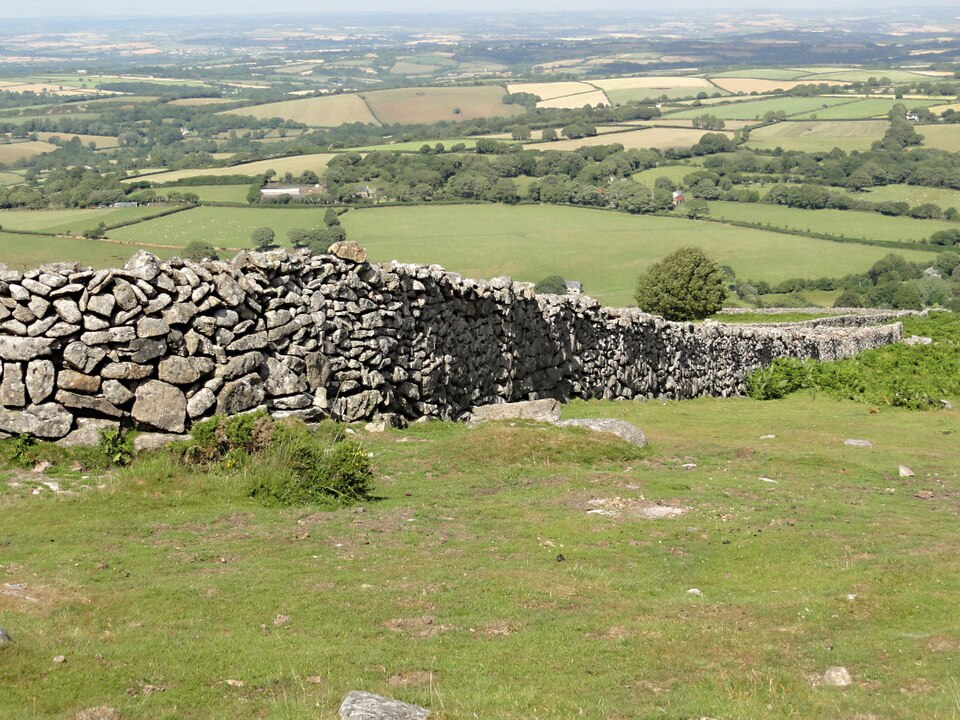
\includegraphics[width=\linewidth]{images/book1/g3-granite-wall.jpg}

{\small Een muur van granietblokken, gebouwd zonder mortel. Foto: Tony
Atkin, Geograph (CC BY-SA 2.0).}
\end{minipage}\hfill
\begin{minipage}[b]{0.49\linewidth}\centering
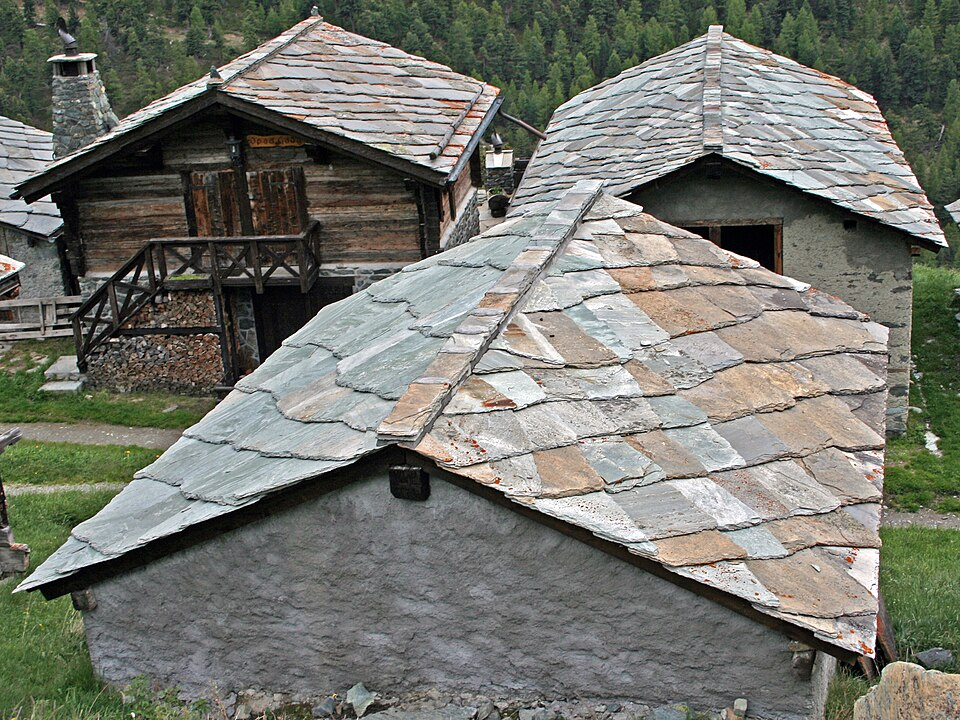
\includegraphics[width=\linewidth]{images/book1/g3-slate-roof.jpg}

{\small Daken van dunne, platte stenen platen in een bergdorp in
Zwitserland. Foto: Michael C. Rygel (CC BY-SA 3.0).}
\end{minipage}
\end{omfigure}

\begin{omfigure}
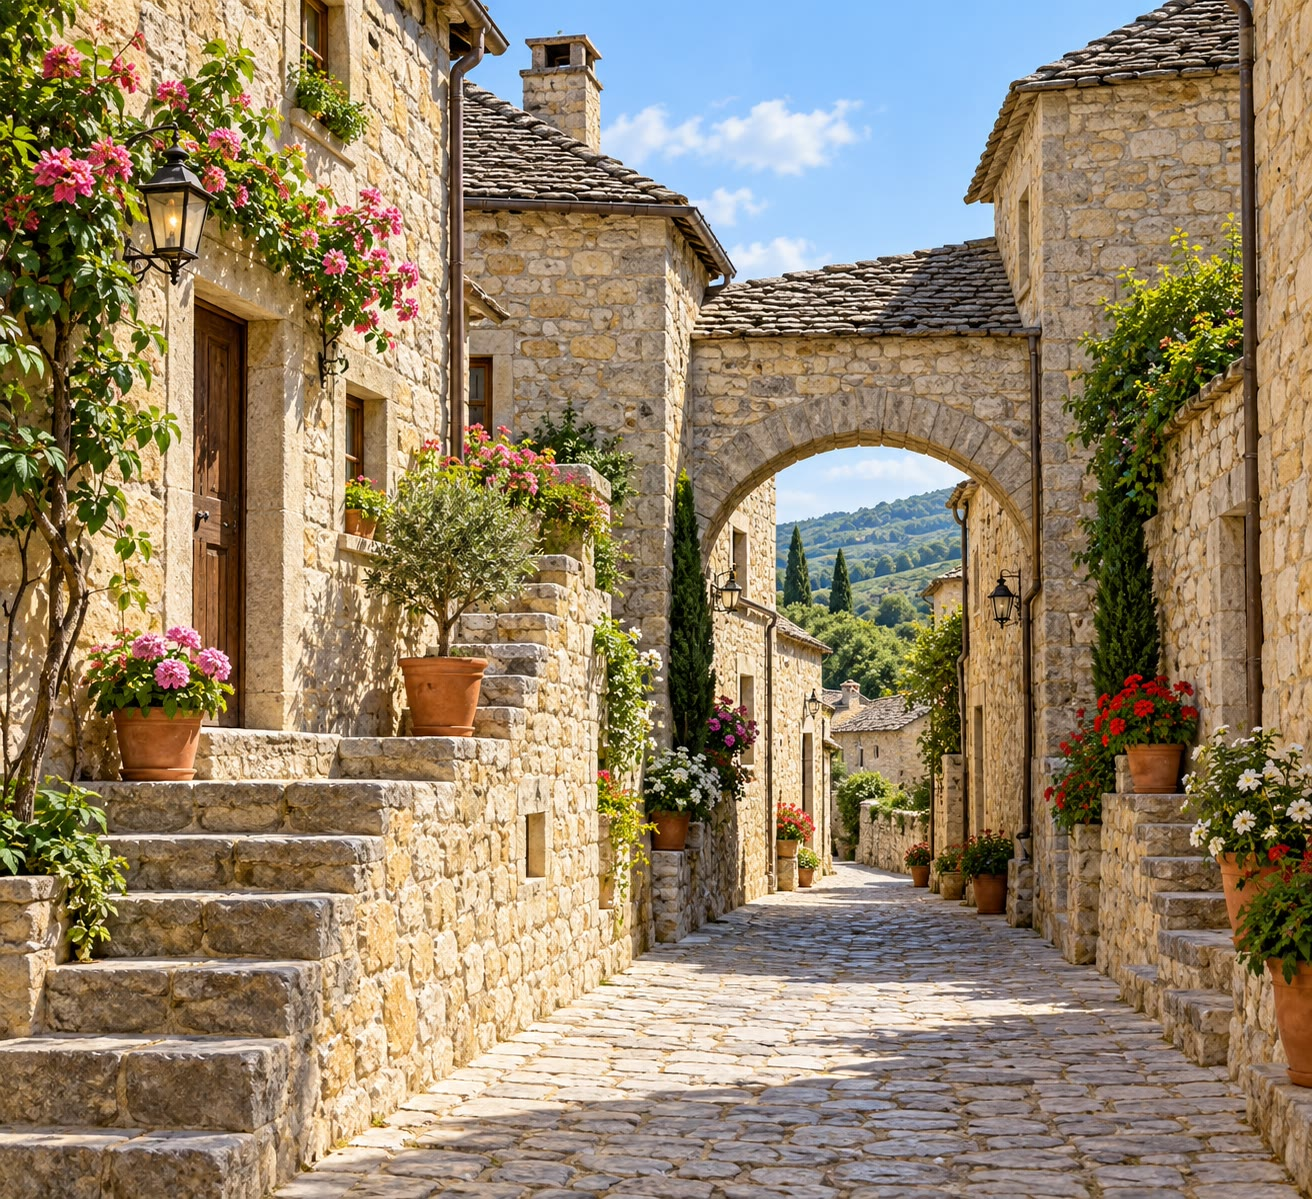
\includegraphics[width=0.6\linewidth]{images/book1/ai/g3-stone-village.jpg}

{\small Een oud dorp, helemaal gebouwd met de steen van de \omterm{def:g1:landscapes-around-us:landform}{heuvel} ernaast.}
\end{omfigure}

Tegenwoordig bouwen we ook met bakstenen, beton en glas. Maar een baksteen
is gemaakt van gebakken klei, beton van \omterm{def:g3:stones-pebbles-sand:sand}{zand}, \omterm{def:g3:stones-pebbles-sand:pebble}{grind} en cement, en glas van
\omterm{def:g3:stones-pebbles-sand:sand}{zand}: ook die komen allemaal uit de \omterm{def:g3:stones-pebbles-sand:rock}{gesteenten} van de Aarde.

\section{Oefeningen}

\begin{exercise}[$\star$]\label{exo:g3:stones-pebbles-sand:1}
Wat is het \omterm{def:g3:stones-pebbles-sand:rock}{vaste gesteente}? Waar kunnen we het zien zonder te graven?
\end{exercise}

\begin{exercise}[$\star$]\label{exo:g3:stones-pebbles-sand:2}
Zet op volgorde van grootte, van klein naar groot: \omterm{def:g3:stones-pebbles-sand:pebble}{kiezel}, \omterm{def:g3:stones-pebbles-sand:sand}{slib},
rotsblok, \omterm{def:g3:stones-pebbles-sand:sand}{zand}.
\end{exercise}

\begin{exercise}[$\star$]\label{exo:g3:stones-pebbles-sand:3}
Een korrel is 1 millimeter groot. Is het \omterm{def:g3:stones-pebbles-sand:sand}{zand} of \omterm{def:g3:stones-pebbles-sand:pebble}{grind}? Een andere korrel
is 3 millimeter groot: \omterm{def:g3:stones-pebbles-sand:sand}{zand} of \omterm{def:g3:stones-pebbles-sand:pebble}{grind}?
\end{exercise}

\begin{exercise}[$\star$]\label{exo:g3:stones-pebbles-sand:4}
Natuurlijk of door mensen gemaakt? Een \omterm{def:g3:stones-pebbles-sand:pebble}{kiezel}; een baksteen; een blok
graniet; een glasplaat; \omterm{def:g3:stones-pebbles-sand:sand}{zand} op een strand.
\end{exercise}

\begin{exercise}[$\star$]\label{exo:g3:stones-pebbles-sand:5}
Waarom heeft een \omterm{def:g3:stones-pebbles-sand:pebble}{kiezel} uit een \omterm{def:g1:landscapes-around-us:water}{rivier} geen scherpe hoeken?
\end{exercise}

\begin{exercise}[$\star$]\label{exo:g3:stones-pebbles-sand:6}
Noem twee \omterm{def:g3:stones-pebbles-sand:building-stone}{bouwstenen} en zeg waarvoor elk wordt gebruikt op de foto's van
dit hoofdstuk.
\end{exercise}

\begin{exercise}[$\star\star$]\label{exo:g3:stones-pebbles-sand:7}
Tom vindt twee stenen van hetzelfde \omterm{def:g3:stones-pebbles-sand:rock}{gesteente}: de ene is scherp, de andere
rond. Welke heeft verder gereisd? Leg uit.
\end{exercise}

\begin{exercise}[$\star\star$]\label{exo:g3:stones-pebbles-sand:8}
Hoeveel centimeter lang is de grootste \omterm{def:g3:stones-pebbles-sand:pebble}{kiezel} op de tekening van de
korrelgrootten? Hoeveel zandkorrels van 2 millimeter passen er naast elkaar
op 1 centimeter?
\end{exercise}

\begin{exercise}[$\star\star$]\label{exo:g3:stones-pebbles-sand:9}
Waar verwacht je \omterm{def:g3:stones-pebbles-sand:sand}{slib} te vinden: in een snelle bergbeek of in een rustige
vijver? Waarom?
\end{exercise}

\begin{exercise}[$\star\star$]\label{exo:g3:stones-pebbles-sand:10}
Bakstenen, beton en glas worden door mensen gemaakt. Waarom kunnen we toch
zeggen dat ze uit de \omterm{def:g3:stones-pebbles-sand:rock}{gesteenten} van de Aarde komen?
\end{exercise}
